%iffalse
\let\negmedspace\undefined
\let\negthickspace\undefined
\documentclass[journal,12pt,onecolumn]{IEEEtran}
\usepackage{cite}
\usepackage{amsmath,amssymb,amsfonts,amsthm}
\usepackage{algorithmic}
\usepackage{graphicx}
\usepackage{textcomp}
\usepackage{xcolor}
\usepackage{txfonts}
\usepackage{listings}
\usepackage{enumitem}
\usepackage{mathtools}
\usepackage{gensymb}
\usepackage{comment}
\usepackage[breaklinks=true]{hyperref}
\usepackage{tkz-euclide} 
\usepackage{listings}
\usepackage{gvv}                                        
\def\inputGnumericTable{}                                 
\usepackage[latin1]{inputenc}                                
\usepackage{color}                                            
\usepackage{array}                                             
\usepackage{longtable}                                       
\usepackage{calc}                                             
\usepackage{multirow}                                         
\usepackage{hhline}                                           
\usepackage{ifthen}                                           
\usepackage{lscape}
\usepackage{multicol}

\newtheorem{theorem}{Theorem}[section]
\newtheorem{problem}{Problem}
\newtheorem{proposition}{Proposition}[section]
\newtheorem{lemma}{Lemma}[section]
\newtheorem{corollary}[theorem]{Corollary}
\newtheorem{example}{Example}[section]
\newtheorem{definition}[problem]{Definition}
\newcommand{\BEQA}{\begin{eqnarray}}
\newcommand{\EEQA}{\end{eqnarray}}
\newcommand{\define}{\stackrel{\triangle}{=}}
\theoremstyle{remark}
\newtheorem{rem}{Remark}
\begin{document}

\bibliographystyle{IEEEtran}
\vspace{3cm}

\title{NCERT -11.16.1.7}
\author{EE224BTECH11044 - Muthyala koushik
}
\maketitle
\bigskip

\renewcommand{\thefigure}{\theenumi}
\renewcommand{\thetable}{\theenumi}
\textbf{\section{PROBABILITY}}

\textbf{Question:}One die of red colour, one of white colour and one of blue colour are placed in a bag. One die is selected at random and rolled, its colour and the number on its uppermost face is noted. Describe the sample space.\\ 

\solution 
\begin{enumerate}
  \item \textbf{Total Number of Possible Outcomes}\\
  Let $X$ be the random variable representing the outcome of the experiment. The sample space is:
  \begin{align}
   S = \{ (C, n) \mid C \in \{R, W, B\},\; n \in \{1, 2, 3, 4, 5, 6\} \}.
  \end{align}
  Since there are 3 colours and 6 numbers per die,
  \begin{align}
    |S| &= 3 \times 6 = 18.
  \end{align}
  
  \item \textbf{Probability Mass Function (PMF)}\\
  Because each die is equally likely to be chosen and every face is equally likely to occur, each outcome in $S$ has the same probability. Thus, the PMF of $X$ is:
  \begin{align}
    P_X(C, n) &= 
    \begin{cases}
      \dfrac{1}{18}, & \text{if } (C, n) \in S, \\
      0, & \text{otherwise.}
    \end{cases}
  \end{align}
  
  \item \textbf{Cumulative Distribution Function (CDF)}\\
  The CDF for the discrete random variable $X$ is defined as
  \begin{align}
    F_X(C, n) &= P\bigl(X \le (C, n)\bigr) \nonumber 
  \end{align}
  If the outcomes are ordered lexicographically (for example, with $R < W < B$ and for each colour, $1 < 2 < \cdots < 6$), and if $(C, n)$ is the $k$-th outcome in this ordering, then:
  \begin{align}
    F_X(C, n) &= \frac{k}{18}.
  \end{align}
  
  \item \textbf{Numerical Solution (Monte Carlo Simulation)}\\
  An alternative approach is to verify these probabilities via a Monte Carlo simulation. By repeatedly simulating the process of randomly selecting a die, rolling it, and recording the outcome, one can estimate the PMF and CDF empirically.
  
\end{enumerate}

\begin{figure}[h]
	\centering
	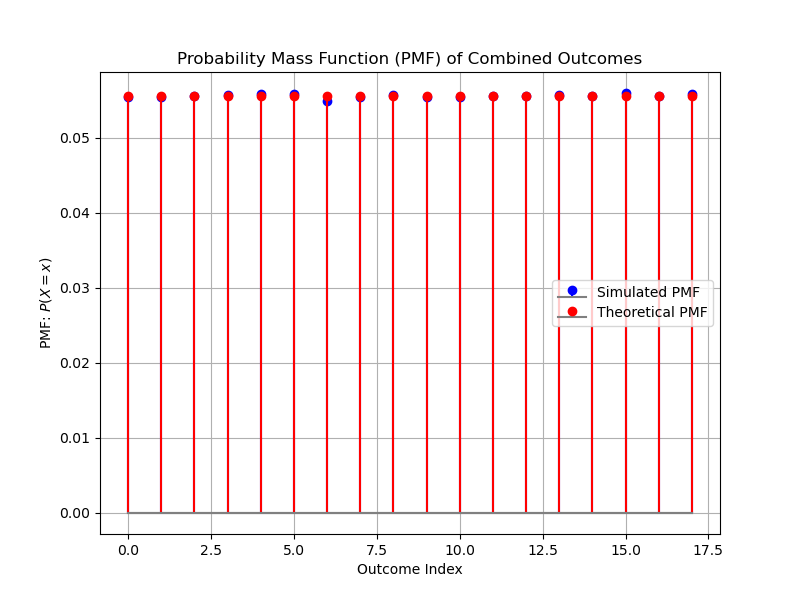
\includegraphics[width=\columnwidth]{figs/pmf_combined_stem.png}
\end{figure}


\begin{figure}[h]
	\centering
	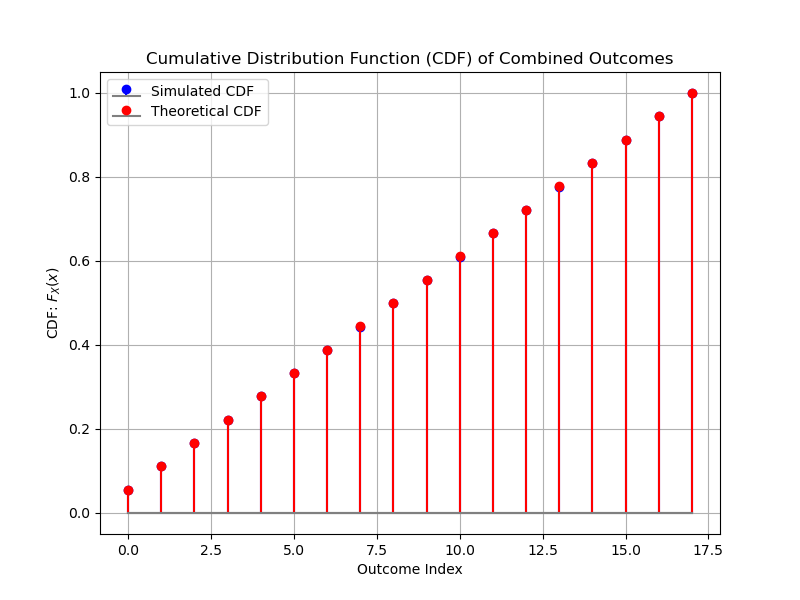
\includegraphics[width=\columnwidth]{figs/cdf_combined_stem.png}
\end{figure}

\end{document}
